\chapter{Ottica geometrica e Fisica moderna}
L'Ottica geometrica studia la propagazione della luce assumendo che si muova in linee rette. Analizza la formazione delle immagini attraverso strumenti ottici come specchi e lenti, basandosi sui fenomeni della riflessione e della rifrazione per spiegare come la luce interagisce con gli oggetti.
\begin{defn}[oggetto]
    L'oggetto per uno strumento ottico è un corpo, puntiforme ed esteso, che emette luce direttamente o diffonde la luce emessa da un altro corpo.
\end{defn}
\begin{defn}[immagine]
    L'immagine è la figura che si crea dai raggi luminosi convergenti dopo aver attraversato lo strumento. L'immagine può essere:
    \begin{enumerate}
        \item reale se i raggi si incontrano fisicamente nei suoi punti;
        \item virtuale se per essa passano i prolungamenti dei raggi, ma non i raggi stessi.
    \end{enumerate}
\end{defn}
\begin{defn}[punti coniugati]
    I punti coniugati sono le posizioni di un punto dell'oggetto e del rispettivo punto dell'immagine.
\end{defn}
\begin{defn}[stigmatismo]
    Se i raggi uscenti da un punto dell'oggetto si incontrano in un solo punto dell'immagine lo strumento è definito stigmatico.
\end{defn}
Lo stigmatismo, condizione essenziale per un a buona definizione dell'immagine, è difficile da ottenere: l'immagine di un punto è quasi sempre estesa, cioè non puntiforme. Nell'ottica geometrica si usa considerare superfici speculari o rifrattive di forma sferica. In queste condizioni, solo se si assumono fasci di raggi di piccola apertura e parassiali, cioè vicini all'asse ottico e formanti con questo angoli molto piccoli, è possibile raggiungere con buona approssimazione una situazione di stigmatismo. Queste approssimazioni sono raccolte sotto il nome di approssimazioni di Gauss.
\begin{axiom}[approssimazioni di Gauss]\hfill
    \begin{enumerate}
        \item Il fascio di raggi che incidono sul sistema ottico deve avere piccola apertura rispetto alle dimensioni del sistema.
        \item I raggi devono essere ragionevolmente parassiali, ovvero avere una piccola inclinazione rispetto all'asse ottico
    \end{enumerate}
\end{axiom}
\begin{defn}[specchi]
    Superfici che la luce incontra su cui può avvenire solo riflessione
\end{defn}
\begin{defn}[diottri]
    Superfici che la luce incontra su cui può avvenire solo trasmissione da un mezzo all'altro.
\end{defn}
Nella costruzione delle immagini negli specchi, nei diottri e nelle lenti è conveniente adottare alcune convenzioni sui segni delle distanze che permettono di trattare tutti i casi senza ambiguità. Allo scopo di semplificare la trattazione degli argomenti è conveniente adottare una convenzione diversa per gli specchi e per i diottri e le lenti.
\begin{axiom}[convenzioni specchi]\hfill
    \begin{enumerate}
        \item La luce proviene sempre da sinistra.
        \item La distanza $p$ di un oggetto P dal vertice V è positiva se l'oggetto si trova a sinistra del vertice, negativa se l'oggetto è a destra di V.
        \item La distanza $q$ dell'immagine Q dal vertice V è negativa se l'oggetto si trova a destra del vertice, positiva se l'oggetto è a sinistra di V.
        \item Il raggio di curvatura $R$ della superficie sferica è negativo se il centro di curvatura si trova a destra di V, positivo se il centro di curvatura si trova a sinistra di V.
        \item Le distanze $y$ dall'asse sono positive per punti al di sopra dell'asse, negative per punti al di sotto, sia per oggetti che per le immagini.
    \end{enumerate}
\end{axiom}
\begin{axiom}[convenzioni diottri e lenti]\hfill
    \begin{enumerate}
        \item La luce proviene sempre da sinistra.
        \item La distanza $p$ di un oggetto P dal vertice V è positiva se l'oggetto si trova a sinistra del vertice, negativa se l'oggetto è a destra di V.
        \item La distanza $q$ dell'immagine Q dal vertice V è positiva se l'oggetto si trova a destra del vertice, negativa se l'oggetto è a sinistra di V.
        \item Il raggio di curvatura $R$ della superficie sferica è positivo se il centro di curvatura si trova a destra di V, negativo se il centro di curvatura si trova a sinistra di V.
        \item Le distanze $y$ dall'asse sono positive per punti al di sopra dell'asse, negative per punti al di sotto, sia per oggetti che per le immagini.
    \end{enumerate}
\end{axiom}
La propagazione dei raggi luminosi avviene tipicamente attraverso mezzi diversi. L'insieme dei mezzi e delle superfici che li separano definisce un sistema ottico. Un sistema ottico può essere composto da diversi elementi posti in successione lungo il percorso dei raggi luminosi.
\begin{figure}[H]
    \centering
    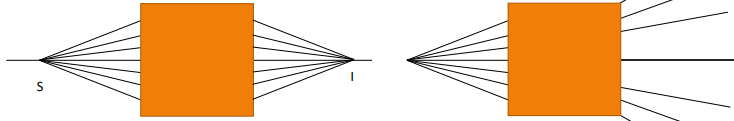
\includegraphics[width=0.75\linewidth]{Immagini ottica/sistemi conv. e div..png}
    \caption{diagramma di un sistema convergente e divergente.}
    \label{fig: sist. conv. e div.}
\end{figure}

In un sistema convergente, i raggi provenienti da sorgente puntiforme convergono in un punto detto immagine. Invece, in un sistema divergente, i raggi divergono e non si forma un'immagine.
\begin{figure}[h]
    \centering
    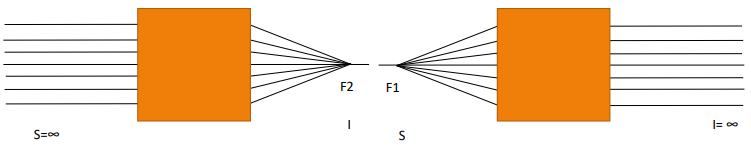
\includegraphics[width=0.75\linewidth]{Immagini ottica/fuochi sist. conv.png}
    \caption{diagramma fuochi di un sistema convergente.}
    \label{fig: fuochi sist. conv.}
\end{figure}

In un sistema convergente sono presenti due fuochi. Il primo fuoco è il punto da cui provengono i raggi la cui immagini si forma all'infinito; il secondo fuoco è il punto in cui i raggi provenienti dall'infinito convergono. Nel caso del secondo fuoco, i raggi possono essere prolungati all'indietro verso la direzione di provenienza. L'immagine si crea quindi a sinistra del sistema ottico, nello spazio degli oggetti. L'immagine che si forma è virtuale.

\section{Diottro sferico}
Un diottro sferico è un sistema ottico costituito da due mezzi omogenei (di indice di rifrazione $n_1$ e $n_2$ diversi, tali che $n_1<n_2$), trasparenti e isotropi, separati da una superficie sferica di raggio $R$. L'asse ottico interseca la superficie sferica nel punto V, riferimento per la misura delle distanze.
\begin{figure}[h]
    \centering
    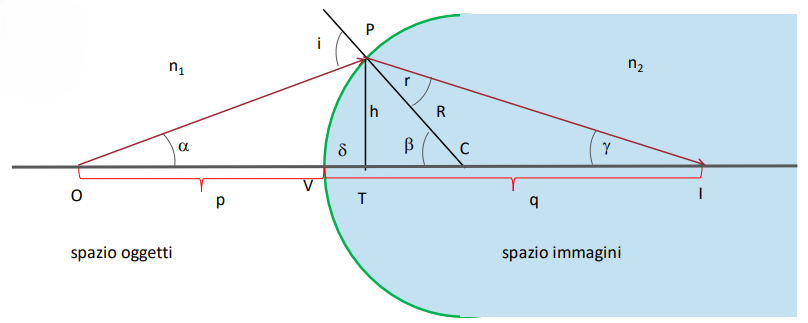
\includegraphics[width=0.8\linewidth]{Immagini ottica/diottro sferico.png}
    \caption{diagramma di un diottro sferico.}
    \label{fig: diottro sferico}
\end{figure}

Per costruire l'immagine si consideri un generico raggio luminoso emesso dalla sorgente O con angolo $\alpha$ rispetto all'asse ottico; esso viene rifratto nel punto P intersecando l'asse ottico nel punto I. Si applica quindi la secondo legge di Snell nel punto P scrivendo 
\begin{equation}
    \label{eq: snell diottro in P}
    n_1\sin{i}=n_2\sin{r}.
\end{equation}
Considerando le proprietà degli angoli si ricava che
\begin{equation}
    \begin{cases}
        \label{eq: angoli i e r diottro}
        i=\alpha+\beta \\
        \beta=r-\gamma\Rightarrow r=\beta-\gamma
    \end{cases}.
\end{equation}
Sostituendo le relazioni del sistema \eqref{eq: angoli i e r diottro} nell'equazione \eqref{eq: snell diottro in P} si ha
\begin{equation}
    \label{eq: snell diottro in P 2}
    n_1\sin{(\alpha+\beta)}=n_2\sin{(\beta-\gamma)}.
\end{equation}
Applicando ora le condizioni dell'approssimazione di Gauss degli assi parassiali si può scrivere l'equazione \eqref{eq: snell diottro in P 2} come
\begin{equation}
    n_1(\alpha+\beta)=n_2(\beta-\gamma)\quad\therefore\quad n_1\alpha +n_2\gamma=\beta(n_2-n_1).
\end{equation}
A questo punto si può applicare ancora l'approssimazione di Gauss, considerando che gli angoli possono essere approssimati alle tangenti
\begin{equation}
\tan{\beta}=\dfrac{h}{R-\delta},\quad\tan{\gamma}=\dfrac{h}{q-\delta},\quad\tan{\alpha}=\dfrac{h}{p+\delta},
\end{equation}
ottenendo pertanto
\begin{equation}
    \label{eq: pre-equazione del diottro}
    \frac{n_1}{p-\delta}+\frac{n_2}{q-\delta}=\frac{n_2-n_1}{R-\delta}.
\end{equation}
Se si assume che il segmento $\delta$ sia trascurabile rispetto a $p$, $q$ e $R$ l'equazione \eqref{eq: pre-equazione del diottro} diventa l'equazione del diottro
\begin{equation}
    \label{eq: equazione del diottro}
    \frac{n_1}{p}+\frac{n_2}{q}=\frac{n_2-n_1}{R}.
\end{equation}
L'equazione del diottro fornisce una relazione tra la posizione $p$ della sorgente e la posizione $q$ dell'immagine indipendentemente dal valore di $\alpha$. In approssimazione di Gauss, il diottro trasforma fasci omocentrici in fasci rifratti omocentrici. L'equazione \eqref{eq: equazione del diottro} è detta anche equazione di Cartesio e i punti di coordinate $p$ e $q$ che la soddisfano sono detti punti coniugati rispetto al diottro.

\paragraph{Fuochi.} Se la posizione $p$ della sorgente tende all'infinito, l'immagine si trova in un punto $F_2$, posto a distanza $f_2$ dal diottro sferico detto secondo fuoco. Se l'immagine si forma a distanza infinita, l'oggetto si trova in un punto $F_1$, detto primo fuoco, a distanza $f_1$ dal diottro e i raggi uscenti da $F_1$ si rifrangono parallelamente all'asse ottico. Dall'equazione \eqref{eq: equazione del diottro} si ricavano i valori di $f_1$ e $f_2$ come
\begin{equation}
    \begin{cases}
        f_2=\lim_{p\to\infty}{q}=R\dfrac{n_2}{n_2-n_1} \\[2ex]
        f_1=\lim_{q\to\infty}{p}=R\dfrac{n_1}{n_2-n_1}
    \end{cases}.
\end{equation}
Dunque, l'equazione \eqref{eq: equazione del diottro} può essere riscritta come
\begin{equation}
    \frac{f_1}{p}+\frac{f_2}{q}=1,
\end{equation}
da cui si ricava che se l'oggetto è posto tra il primo punto focale e l'infinito ($p> f_1$), esso fornisce un'immagine reale, mentre fornisce un'immagine virtuale quando è posta tra la superficie del diottro e il primo fuoco ($p< f_1$).
\section{Lenti sottili}
Due superfici diottriche aventi lo stesso asse individuano tre regioni distinte: la luce proveniente da sinistra si propaga nel primo mezzo avente indice di rifrazione $n_1$, viene trasmessa dal primo diottro e attraversa il mezzo con indice di rifrazione $n_2$ e infine, dopo la trasmissione al secondo diottro, si propaga nel mezzo con indice di rifrazione $n_3$. Le superfici diottriche possono essere piane o sferiche, convergenti o divergenti. Il mezzo avente indice di rifrazione $n_2$ si chiama lente semplice. Si trattano in particolare casi in cui $n_1=n_3$ e le lenti sono sottili, ovvero con superfici diottriche molto vicine.
\begin{figure}[h]
    \centering
    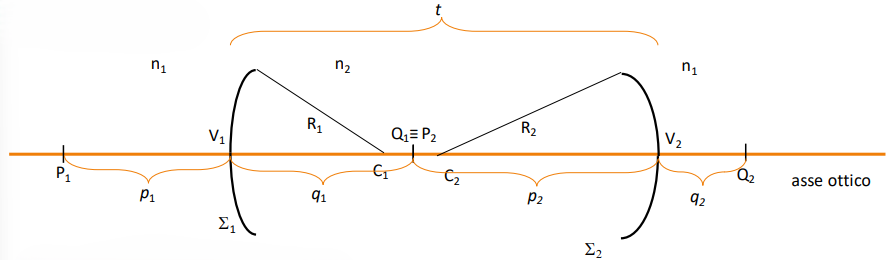
\includegraphics[width=0.95\linewidth]{Immagini ottica/lenti sottili.png}
    \caption{diagramma di una lente sottile.}
    \label{fig: lente sottile}
\end{figure}

Le equazioni dei due diottri, assumendo che l'immagine generata dal primo diventi oggetto del secondo, sono
\begin{equation}
    \begin{cases}
        \dfrac{n_1}{p_1}+\dfrac{n_2}{q_1}=\dfrac{n_2-n_1}{R_1} \\[2ex]
        \dfrac{n_2}{t-q_1}+\dfrac{n_1}{q_2}=\dfrac{n_1-n_2}{R_2},
    \end{cases}
\end{equation}
dove per costruzione si ha $p_2=t-q_1$. Supponendo che $t$ sia trascurabile rispetto alle altre distanze e sommando membro a membro si ottiene
\begin{equation}
    \frac{1}{p_1}+\frac{1}{q_2}=\frac{n_2-n_1}{n_1}\left(\frac{1}{R_1}-\frac{1}{R_2}\right).
\end{equation}
Definendo quindi $p_1=p$ come la distanza dell'oggetto e $q_2=q$ come la distanza immagine si ottiene
\begin{equation}
    \label{eq: eq. costruttore lenti}
    \frac{1}{p}+\frac{1}{q}=\frac{n_2-n_1}{n_1}\left(\frac{1}{R_1}-\frac{1}{R_2}\right)=\dfrac{1}{f},
\end{equation}
dove $f_1=f_2=f$.
L'equazione \eqref{eq: eq. costruttore lenti} permette di definire i fuochi di una lente sottile
\begin{equation}
    \begin{cases}
        f_2=\lim_{p\to\infty}{q}=\dfrac{1}{f_2}=\dfrac{n_2-n_1}{n_1}\left(\dfrac{1}{R_1}-\dfrac{1}{R_2}\right) \\[2ex]
        f_1=\lim_{q\to\infty}{p}=\dfrac{1}{f_1}=\dfrac{n_2-n_1}{n_1}\left(\dfrac{1}{R_1}-\dfrac{1}{R_2}\right)
    \end{cases}
\end{equation}
Inoltre, dall'equazione \eqref{eq: eq. costruttore lenti} si ricava la legge dei punti coniugati
\begin{equation}
    \label{eq: legge dei punti coniugati}
    \frac{1}{p}+\frac{1}{q}=\frac{1}{f}.
\end{equation}
\begin{defn}[potere diottrico]
    Il potere diottrico $P$ di una lente è l'inverso della distanza focale $f$ espressa in metri. La sua unità di misura è la diottria.
\end{defn}

\paragraph{Sistemi di lenti sottili.} Si considerino due lenti sottili poste in successione di focali rispettivamente $f_1$ e $f_2$. Assumendo che l'immagine creata dalla prima lente diventi oggetto della seconda e ricordando che 
\begin{equation}
    \begin{cases}
    \label{eq: sistema lenti a contatto}
        \dfrac{1}{f_1}=\dfrac{1}{p_1}+\dfrac{1}{q_1} \\[2ex]
        \dfrac{1}{f_2}=\dfrac{1}{p_2}+\dfrac{1}{q_2},
    \end{cases}
\end{equation}
dove $p_2=d-q_1$. Sommando le equazioni del sistema \eqref{eq: sistema lenti a contatto} si trova
\begin{equation}
    \label{eq: eq: somma sistema lenti a contatto}
    \dfrac{1}{f_1}+\dfrac{1}{f_2}=\dfrac{1}{p_1}+\dfrac{1}{q_1}+\dfrac{1}{d-q_1}+\dfrac{1}{q_2}.
\end{equation}
Se $d=0$, ovvero se le lenti sono a contatto, l'equazione \eqref{eq: eq: somma sistema lenti a contatto} diventa
\begin{equation}
    \dfrac{1}{f_1}+\dfrac{1}{f_2}=\dfrac{1}{p}+\dfrac{1}{q},
\end{equation}
dove $p$ e $q$ rappresentano la distanza
oggetto e immagine del sistema. Si definisce pertanto la focale $f$ del sistema di lenti a contatto per cui vale
\begin{equation}
    \label{eq: focale sistema lenti a contatto}
    \frac{1}{f}=\dfrac{1}{f_1}+\dfrac{1}{f_2}.
\end{equation}

\paragraph{Ingrandimento.} Si consideri una lente sottile. Come mostrato in figura \ref{fig: ingrandimento}, indicando con $V$ il centro della lente sottile, dato che il triangolo formato da $h_o$, la distanza oggetto-V e il raggio passante per il centro, è simile al triangolo formato da $h_i$, la distanza immagine-V e il medesimo raggio, si può scrivere
\begin{equation}
    \label{eq: ingrandimento}
    \frac{h_i}{h_o}=\frac{-q}{p}=G,
\end{equation}
dove $G$ è appunto il coefficiente di ingrandimento. Se $G>0$, allora l'immagine è dritta rispetto all'oggetto, mentre se $G<0$ l'immagine risulta capovolta.
\begin{figure}[h]
    \centering
    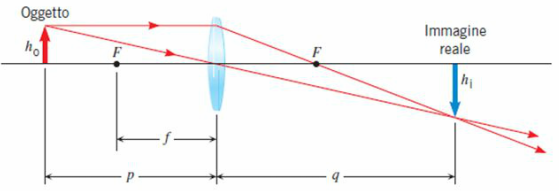
\includegraphics[width=0.65\linewidth]{Immagini ottica/ingrandimento.png}
    \caption{diagramma per ingrandimento di una lente sottile.}
    \label{fig: ingrandimento}
\end{figure}

\section{Aberrazioni}
\paragraph{Cromatismo.} Uno dei difetti ottici più semplici da riconoscere è l'aberrazione cromatica. Gli oggetti luminosi presentano aloni colorati più o meno diffusi. I colori più probabili da osservare sono il rosso e il blu, l'uno intra e l'altro extrafocale. Il problema nasce dall'impossibilità per una lente di mettere a fuoco tutte le lunghezze d'onda nello stesso piano focale per via della dispersione che la luce subisce attraversando materiali di densità ottica diversa. In pratica quando si fa il fuoco con un rifrattore acromatico di fatto si fa il fuoco nel verde sacrificando il rosso e il blu che finiscono sfuocati. Per correggere questo difetto ottico si usano i “doppietti acromatici”, ossia coppie di lenti convergente-divergente opportunamente lavorate.

\paragraph{Sfericità.} Quando dei raggi paralleli all'asse ottico incidono su una lente con superfici sferiche, solo i raggi parassiali passano per il fuoco parassiale $F$. Invece, i raggi più lontani dall'asse vengono deviati in punti più distanti rispetto ad $F$, mentre quelli più vicini all'asse vengono deviati in punti antecedenti $F$, come mostrato in figura \ref{fig: sfericità}. Questo effetto prende il nome di aberrazione sferica. A causa di questa aberrazione, l'immagine di un punto luminoso non risulta essere ancora un punto, ma una macchia luminosa di forma circolare, spesso circondata da un alone di luce. Tra tutti i punti lungo l'asse, ce n'è uno in cui il diametro di questa macchia è minimo, detto cerchio di minima confusione.
\begin{figure}[h]
    \centering
    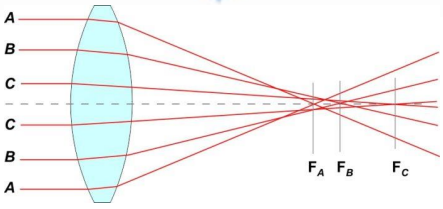
\includegraphics[width=0.5\linewidth]{Immagini ottica/sfericità.png}
    \caption{effetto della sfericità.}
    \label{fig: sfericità}
\end{figure}

\paragraph{Coma.} Questo difetto ottico avviene quando l'oggetto è lontano dall'asse ottico e i raggi sono tra di loro paralleli, ma inclinati rispetto all'asse della lente. Quando tali raggi incidenti attraversano la lente lontano dall'asse, i raggi rifratti non si incontrano tutti nello stesso punto, poiché la superficie della lente può essere approssimata con un piano solo nella zona parassiale. Di conseguenza, a seconda della distanza del raggio dal centro della lente la corrispondente immagine sarà un cerchio di raggio diverso e diversa distanza dall'asse. Per correggere questo difetto ottico si deve impiegare un diaframma in una posizione tale da limitare l'area della lente su cui i raggi obliqui sono incidenti.

\paragraph{Astigmatismo.} Questo difetto ottico avviene quando l'oggetto è vicino e fuori asse. Considerando un singolo punto dell'oggetto e seguendo il percorso dei raggi sul piano tangenziale e su quello sagittale:
\begin{itemize}
    \item i fasci di luce che incidono lungo il meridiano tangenziale AA' convergeranno nel punto T, detto immagine primaria;
    \item i fasci di luce che incidono lungo il meridiano sagittale BB' focalizzano nel punto S, detto immagine secondaria.
\end{itemize}
Nel punto T si trova il fuoco dei raggi tangenziali. I fasci sagittali non saranno ancora a fuoco, si vede una linea detta ``focalina'' o immagine tangenziale. Invece, nel punto S si trova il fuoco dei raggi sagittali. Il fascio dei raggi tangenziali diverge. Anche qui si vede un'immagine della focalina sagittale. La distanza tra le focaline è detta intervallo di Sturm. Quindi, la miglior immagine del punto P si può vedere a metà tra T e S ed è detto cerchio di minima confusione. Per correggere questo difetto ottico si devono usare lenti cilindriche; i sistemi corretti si dicono sistemi anastigmatici.
\begin{figure}[h]
    \centering
    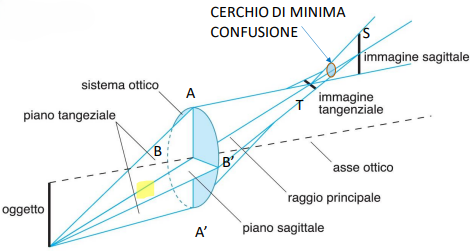
\includegraphics[width=0.7\linewidth]{Immagini ottica/astigmatismo.png}
    \caption{effetto dell'astigmatismo.}
    \label{fig: astigmatismo}
\end{figure}

\paragraph{Distorsioni.} Questo difetto ottico riguarda l'aberrazione della forma dell'immagine di un oggetto esteso dovuta al fatto che l'ingrandimento $G$ dipende dalla distanza del punto oggetto dall'asse $d$, si presentano due casi:
\begin{enumerate}
    \item se $G$ aumenta con $d$ si ha una distorsione a cuscinetto;
    \item se $G$ diminuisce con $d$ si ha una distorsione a barilotto.
\end{enumerate}
Per correggere questo difetto ottico si deve usare un sistema detto doppietto ortoscopico, formato da una coppia di lenti e un diaframma.
\begin{obs}
Per diaframma si intende una limitazione meccanica che riduce in una certa misura la quantità di radiazione che incide su un sistema ottico o che da esso viene trasmessa limitando l'apertura dei fasci. Il diaframma può essere posizionato all'ingresso del sistema, tra lenti all'interno di esso oppure in uscita.
\end{obs}

\section{Banco ottico}
Le ipotesi consistono nell'assumere che il sistema sia un sistema ottico centrato e che valgano le approssimazioni di Gauss. L'esperienza si articola in due parti contraddistinte da due obiettivi differenti: determinare la distanza focale tramite l'equazione \eqref{eq: legge dei punti coniugati} di una lente convergente e di un'altra divergente; verificare la legge dell'ingrandimento tramite l'equazione \eqref{eq: ingrandimento}.
\begin{figure}[h]
    \centering
    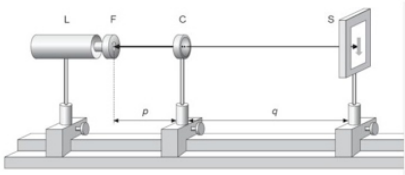
\includegraphics[width=0.7\linewidth]{Immagini ottica/apparato banco ottico.png}
    \caption{banco ottico.}
    \label{fig: banco ottico}
\end{figure}

Per determinare la focale della lente convergente e di quella divergente, i passi da seguire sono:
\begin{enumerate}
    \item lasciare fissa la distanza oggetto-lente $p$ e di cercare ripetutamente la posizione dello schermo che mette a fuoco l'immagine, variando la distanza lente-schermo $q$. Eseguire un numero di misurazioni tale che sia possibile valutare la distribuzione di $q$. Ripetere l'esercizio dopo aver ruotato la lente di 180°. Si valuti la compatibilità statistica delle distanze focali prima e dopo la rotazione della lente. Si facciano le considerazioni del caso riguardo alle distribuzioni ottenute. Si valuti la lunghezza focale della lente;
    \item variare alcune volte la distanza oggetto-lente $p$. Per ogni valore di $p$, si cerchi ripetutamente il valore di $q$ per cui l'immagine è a fuoco sullo schermo. Riportare le misure nel piano avente $1/p$ sulle ascisse e $1/q$ sulle ordinate. Eseguire un fit lineare ed estrarne la lunghezza focale;
    \item con lo stesso metodo, si misuri la lunghezza focale di una lente divergente (lunghezza focale negativa). Occorre combinarla con una lente convergente in modo che la focale risultante sia positiva. In particolare, per determinare la focale $f_{div}$ si deve usare la formula
    \begin{equation}
            \frac{1}{f_{sist}}=\frac{1}{f_{conv}}+\frac{1}{f_{div}}.
        \end{equation}
    \end{enumerate}
Per verificare la legge dell'ingrandimento ricavata in \eqref{eq: ingrandimento}, i passi da seguire sono:
\begin{enumerate}
    \item si misura la lunghezza di un particolare dell'immagine;
    \item si misurano diversi valori di $p$ e $q$;
    \item per ogni coppia di dati si misura la lunghezza dello stesso particolare sullo schermo;
    \item si confrontano i valori di $G$ ottenuti con la formula \eqref{eq: ingrandimento}.
\end{enumerate}

\section{Spettroscopio di Kirchhoff-Bunsen}
\paragraph{Prisma in deviazione minima.} Un modo molto semplice per disperdere la luce è tramite un prisma di vetro. Da considerazioni geometriche sugli angoli in figura \ref{fig: prisma} si trova che
\begin{equation}
    \begin{cases}
    \label{eq: sistema prisma}
        \theta=\pi-(i-r)-(i'-r') \\
        D=\pi-\theta=(i-r)+(i'-r') \\
        \beta+r=\gamma+r'=\pi/2 \\
        \alpha+\beta+\gamma=\pi \\
        \alpha=r+r'
    \end{cases}.
\end{equation}
\begin{figure}[H]
    \centering
    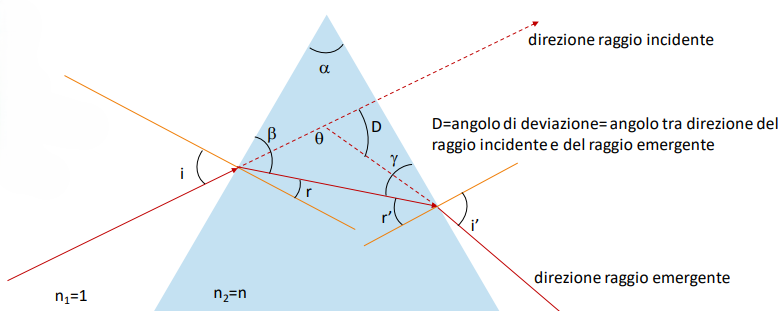
\includegraphics[width=0.85\linewidth]{Immagini ottica/Prisma.png}
    \caption{dispersione della luce tramite un prisma.}
    \label{fig: prisma}
\end{figure}

Ora considerando la penultima equazione del sistema \eqref{eq: sistema prisma} e sostituendo i valori di $\gamma$ e $\beta$ del sistema \eqref{eq: sistema prisma} si trova
\begin{equation}
    \label{eq: angolo alpha prisma}
    \alpha=\pi-\left(\frac{\pi}{2}-r\right)-\left(\frac{\pi}{2}-r'\right)=r+r'.
\end{equation}
Pertanto, si ha
\begin{equation}
    \label{eq: andolo d prisma}
    D=i+i'-\alpha=i+i'-r-r'.
\end{equation}
Ora partendo dalle equazioni \eqref{eq: angolo alpha prisma} e \eqref{eq: andolo d prisma} si può applicare la seconda legge di Snell per elaborare ulteriormente il risultato. Quindi, da
\begin{equation}
    \label{eq: sistema prisma 3}
    \begin{cases}
        \alpha=r+r' \\
        \sin{i}=n\sin{r} \\
        \sin{i'}=n\sin{r'}
    \end{cases},
\end{equation}
si ha 
\begin{equation}
    \sin{i'}=n\sin{r'}=n\sin{(\alpha-r)}=n(\sin{\alpha}\cos{r}-\cos{\alpha}\sin{r}),
\end{equation}
e sostituendo $\sin{r}$ con la prima equazione del sistema \eqref{eq: sistema prisma 3} si ottiene
\begin{equation}
    \begin{split}
    \label{eq: sin i' prisma}
    \sin{i'}&=n\left(\sin{\alpha}\sqrt{1-\frac{\sin^2{i}}{n^2}}-\cos{(\alpha)}\frac{\sin{i}}{n}\right) \\
    &=\sin{\alpha}\sqrt{n^2-\sin^2{i}}-\cos{\alpha}\sin{i}.
    \end{split}    
\end{equation}
Sostituendo quindi l'equazione \eqref{eq: sin i' prisma} nell'equazione \eqref{eq: andolo d prisma} si trova
\begin{equation}
    \label{eq: finale angolo d prisma}
    D=i-\alpha+\arcsin{\left(\sin{\alpha}\sqrt{n^2-\sin^2{i}}-\cos{\alpha}\sin{i}\right)}.
\end{equation}
L'equazione \eqref{eq: finale angolo d prisma} è molto utile per esigenze sperimentali in quanto l'unica grandezza da misurare per conoscere l'angolo di deviazione $D$ è l'angolo di incidenza $i$. Sempre da questa equazione si ricava
\begin{equation}
    \label{eq: indice rifrazione prisma generale}
    n=\sqrt{ \left(\sin{(D+\alpha-i)}+\sin{i}\cos{\alpha}\right)^2\frac{1}{\sin^2{\alpha}}+\sin^2{i}}
\end{equation}
Per semplificare la relazione \eqref{eq: indice rifrazione prisma generale}, si può cercare la condizione di incidenza per cui l'angolo $D$ è minimo. Per fare ciò si minimizza l'equazione \eqref{eq: andolo d prisma}. Si parte quindi dalle relazioni
\begin{equation}
    \begin{cases}
    \label{eq: sistema prisma min. dev.}
        D=i+i'-\alpha \\
        r'=\alpha-r \\
        \sin{i}=n\sin{r} \\
        n\sin{r'}=\sin{i'}
    \end{cases}.
\end{equation}
Differenziando il sistema \eqref{eq: sistema prisma min. dev.} si trova
\begin{equation}
    \begin{cases}
        dD=di+di' \\
        dr'=-dr \\
        \cos{(i)}di=n\cos{(r)}dr \\
        n\cos{(r')}dr'=\cos{(i')}di'
    \end{cases},
\end{equation}
da cui
\begin{equation}
    \begin{cases}
        di'=n\dfrac{\cos{r'}}{\cos{i'}}dr' \\[2ex]
        dr=\dfrac{1}{n}\dfrac{\cos{i}}{\cos{r}}di
    \end{cases}.
\end{equation}
Ora da $dr'=-dr$ si ha
\begin{equation}
    di'=n\frac{\cos{r'}}{\cos{i'}}dr'=-n\frac{\cos{r'}}{\cos{i'}}\frac{1}{n}\frac{\cos{i}}{\cos{r}}di=-\frac{\cos{r'}}{\cos{i'}}\frac{\cos{i}}{\cos{r}}di,
\end{equation}
che sostituito in $dD=di+di'$ restituisce
\begin{equation}
    \label{eq: dD/di}
    \frac{dD}{di}=1-\frac{\cos{r'}}{\cos{i'}}\frac{\cos{i}}{\cos{r}}.
\end{equation}
Minimizzando ora \eqref{eq: dD/di} ponendo $dD/di=0$, si ha la condizione
\begin{equation}
    \cos{i}\cos{r'}=\cos{r}\cos{i'},
\end{equation}
la quale è soddisfatta quando $i=i'$ e $r=r'$, ovvero quando il raggio viaggia parallelo alla base del prisma equilatero. Dunque, considerando l'equazione \eqref{eq: andolo d prisma} ponendo il prisma in deviazione minima si ha che l'angolo di incidenza è
\begin{equation}
    i=\frac{D_m+\alpha}{2},\quad \alpha=2r,
\end{equation}
che sostituito in $\sin{i}=n\sin{r}$ restituisce infine
\begin{equation}
    \label{eq: indice rifrazione prisma dev. min.}
    n=\frac{\sin{\left(\dfrac{D_m+\alpha}{2}\right)}}{\sin{(\alpha/2)}}.
\end{equation}
Ottenuti questi risultati, le ipotesi dell'esperienza consistono nel considerare l'angolo al vertice $\alpha$ noto dal costruttore e di posizionarsi con il prisma in condizione di deviazione minima, provando a posizionare il reticolo il più perpendicolare possibile al collimatore; per farlo bisogna verificare che, preso un massimo, questo si trovi allo stesso angolo a sinistra e a destra del collimatore. L'esperienza si articola in due parti con l'obiettivo di stimare l'indice di rifrazione $n$ del prisma e misurare le lunghezze d'onda componenti lo spettro del mercurio.
\begin{figure}[H]
    \centering
    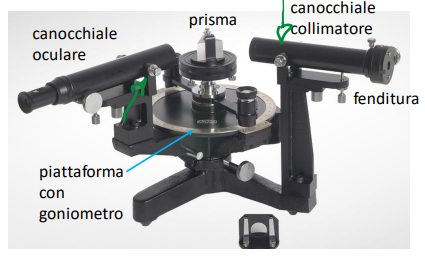
\includegraphics[width=0.55\linewidth]{Immagini ottica/apparato spettr..png}
    \caption{spettroscopio di Kirchhoff-Bunsen.}
    \label{fig: spettroscopio}
\end{figure}

Per determinare la posizione di deviazione minima, i passi da seguire sono:
\begin{enumerate}
    \item in assenza del prisma, si ruota il cannocchiale inquadrando la riga corrispondente alla fenditura. Poi si ripone il prisma sulla piattaforma e si seguono le righe spettrali fino a che queste non raggiungono la posizione di minimo. Questo accade quando si nota che le righe ``invertono il proprio moto'';
    \item si misurano le posizioni angolari di ciascuna riga dello spettro in questa condizione;
    \item l'angolo di deviazione $D_m$ è dato dalla differenza tra la posizione del raggio non deviato e quella delle righe, per cui $D_m=\ang{360}-\theta$;
    \item per calcolare le stime di $n$ si usa l'equazione \eqref{eq: indice rifrazione prisma dev. min.};
    \item ottenuti i valori di $n$ per le diverse lunghezze d'onda si opera una regressione di $n(\lambda)$ con la legge di Cauchy
    \begin{equation}
        n(\lambda)=A+\frac{B}{\lambda^2},\quad A,B\in\mathbb{R}.
    \end{equation}
\end{enumerate}
Per determinare l'indice di rifrazione del prima, i passi da seguire sono:
    \begin{enumerate}
        \item si sostituisce il prisma con il reticolo e si guarda nel cannocchiale dove si vedono $N$ spettri, uno per ogni ordine massimo, a destra e a sinistra della riga centrale (per ordini superiori a $m=2$ le righe di diversi ordini si possono sovrapporre);
        \item analogamente a quanto fatto con il prisma si misurano le posizioni angolari di alcune righe per gli ordini $m=1,2,3$;
        \item dalla formula $p\sin{\theta}=m\lambda$ si ricavano i valori di $\lambda$ di ogni riga misurata.
    \end{enumerate}
Per determinare lo spettro del mercurio, i passi da seguire sono:
    \begin{enumerate}
        \item si avvicina la fibra ottica alla lampada a vapori di mercurio e si osservano i picchi di lunghezza d'onda riportati dal software;
        \item si confrontano i valori dello spettrofotometro con quelli ricavati con lo spettroscopio.
    \end{enumerate}
\begin{obs}
    Il reticolo di diffrazione è un componente ottico costituito solitamente da una lastra di vetro sulla cui superficie è incisa una trama di linee parallele, uguali ed equidistanti, a distanze confrontabili con la lunghezza d'onda della luce. Sfrutta il principio ottico dell'interferenza di moltissimi fasci di luce che abbiano una precisa relazione di fase tra loro, ottenuti facendo passare la luce attraverso un gran numero di fenditure regolari. Se la sorgente è policromatica per ogni massimo si formeranno $N$ picchi, uno per ciascuna componente dello spettro. Quindi, si formeranno $M$ spettri, uno per ogni ordine di massimo.
\end{obs}

\section{Interferometro}
Le ipotesi consistono nel conoscere lo spostamento dello specchio tramite la vite micrometrica e il goniometro dell'interferometro, insieme allo spessore della lastra di vetro e alla misura della camera a vuoto della pompa. L'esperienza si articola in tre parti in cui si vuole: misurare la lunghezza d'onda del laser He-Ne, stimare l'indice di rifrazione della lastra di vetro; stimare l'indice di rifrazione dell'aria.
\begin{figure}[H]
    \centering
    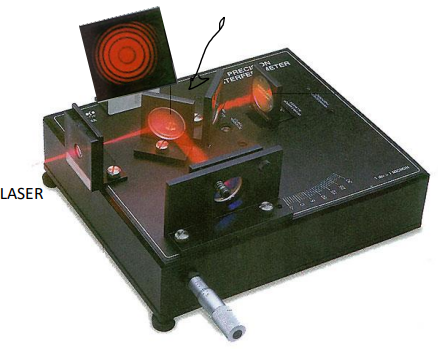
\includegraphics[width=0.5\linewidth]{Immagini ottica/interferometro.png}
    \caption{interferometro laser.}
    \label{fig: interferometro}
\end{figure}

\noindent
Per misurare la lunghezza d'onda del laser He-Ne, i passi da seguire sono:
\begin{enumerate}
    \item si varia la posizione dello specchio mobile e si contano le frange di interferenza che scompaiono (o appaiono, a seconda della direzione dello spostamento) nel centro della figura di interferenza; 
    \item si conta un numero $N$ fisso di frange (80 circa) e si registra lo spostamento $\Delta x$ indicato dalla vite micrometrica;
    \item ripetendo la misura $M$ volte, si ricava la lunghezza d'onda da
    \begin{equation}
        \lambda=\frac{2\Delta x}{N}.
    \end{equation}
\end{enumerate}
Per stimare l'indice di rifrazione della lastra di verto, i passi da seguire sono:
\begin{enumerate}
        \item si varia l'inclinazione della lastra rispetto al raggio incidente: il cambiamento di cammino ottico indotto dall'inclinazione fa muovere le frange di interferenza;
        \item di nuovo si conta un numero $N$ fisso di frange scomparse o apparse (50 circa) e si registra l'angolo $\theta$, misurato con un goniometro con precisione di un decimo di grado; 
        \item si ripete la misura $M$ volte e si ricava $n_{vetro}$ tramite la formula
        \begin{equation}
        n_{vetro}=\frac{(2t-N\lambda)(1-\cos{\theta})}{2t(1-\cos{\theta})-N\lambda},
    \end{equation}
    dove $t$ è lo spessore della lastra.
    \end{enumerate}
Per stimare l'indice di rifrazione dell'aria, i passi da seguire sono:
\begin{enumerate}
    \item si introduce su uno dei bracci dell'interferometro una camera, entro la quale è possibile variare la pressione usando una pompa a mano misurabile con un manometro con precisione di 100 mbar;
    \item Il manometro misura la differenza di pressione tra l'atmosfera e l'interno della camera. Un pulsante consente di far entrare o uscire lentamente l'aria dalla camera. Il procedimento consiste nel portare la camera ad un valore di $\Delta p$ desiderato;
    \item la variazione di pressione induce una variazione di indice di rifrazione, muovendo le frange di interferenza;
    \item si conta quante frange $N$ scompaiono (o appaiono) per una data variazione di pressione $\Delta p$. Si costruisce il grafico avente $\Delta p$ in ascisse e $N$ in ordinate;
    \item Conoscendo la lunghezza $d$ della camera a vuoto, si estrapola il valore del coefficiente angolare $m$ della retta e si calcola $n_{aria}$ dell'aria tramite la formula
    \begin{equation}
        n_{aria}=1+\frac{\lambda m}{2d}.
    \end{equation}
\end{enumerate}

\section{Polarimetro di Laurent}
L'esperienza si basa sull'utilizzo di sostanze otticamente attive e sul fenomeno consistente nella rotazione del piano di polarizzazione in uscita dalla soluzione contente tali sostanze, rispetto a quello in entrata. Inoltre, sfruttando il fenomeno della birifrangenza e il fatto che il vettore elettrico del raggio ordinario e straordinario vibrano in direzioni perpendicolari tra loro, è possibile ottenere un'onda polarizzata linearmente facendo in modo che uno dei fasci subisca riflessione totale. 

Le ipotesi dell'esperienza consistono nell'assumere che le misure si svolgono a temperatura costante e che la lampada al sodio sia una sorgente monocromatica. L'esperienza si articola quindi in due parti in cui si vuole stimare la concentrazione di fruttosio e saccarosio in alcune soluzioni acquose e verificare la legge di Malus tramite un filtro polarizzatore.
\begin{figure}[h]
    \centering
    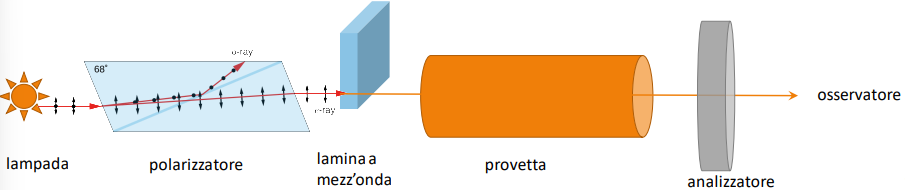
\includegraphics[width=0.9\linewidth]{Immagini ottica/polarizzatore.png}
    \caption{diagramma polarimetro di Laurent.}
    \label{fig: polarimetro}
\end{figure}

L'azione del polarimetro di Laurent si riassume in breve così: la luce generata dalla lampada al sodio viene polarizzata linearmente dal prisma di Nicol, metà di questo fascio attraversa una lamina a mezz'onda, mentre l'altra metà prosegue senza variazioni dello stato di polarizzazione; entrambi i fasci attraversano quindi un analizzatore. Ora, per determinare la concentrazione di saccarosio e fruttosio, i passi da seguire sono:
\begin{enumerate}
    \item si osserva che campi sono illuminati in modo diverso corrispondono all'effetto dell'analizzatore sui fasci;
    \item si ruota l'analizzatore fino a che i campi hanno la stessa illuminazione nella condizione di ``bassa illuminazione'' e si misura l'angolo $\theta$ al quale ciò avviene, una sola volta per il polarimetro scarico ($\theta'$), le altre volte con le provette di soluzione acquosa;
    \item sapendo che l'angolo $\alpha$ di rotazione del piano di polarizzazione è $\alpha=\theta-\theta'$ per il saccarosio, mentre $\alpha=(\theta-\theta')-\ang{180}$ per il fruttosio, si usa la legge di Biot
    \begin{equation}
        \label{eq: legge di biot}
        \alpha=kcl,
    \end{equation}
    dove $k$ è il potere rotatorio specifico della sostanza, $c$ è la concentrazione e $l$ è la lunghezza della provetta;
    \item noto $\alpha$ si stimano i valori di $c$ per diversi campioni.
\end{enumerate}
Per verificare la legge di Malus, i passi da seguire sono:
\begin{enumerate}
    \item si verifica che il fascio sia polarizzato linearmente controllando che siano visibili zeri di luce ruotando in polarizzatore di 360°. In caso contrario, si aggiunge un filtro polarizzante tra laser e analizzatore;
    \item si misura la corrente per ogni angolo, si graficano i dati e si effettua una regressione con la legge di Malus $I=I_0\cos^2{\theta}$.
\end{enumerate}

\section{Esperienza effetto fotoelettrico}
L'ipotesi dell'esperienza consiste solamente nel conoscere le lunghezze d'onda dei LED, mentre l'obiettivo di quest'ultima consiste nello stimare la constante di Planck $h$. Per farlo, i passi da seguire sono:
\begin{enumerate}
    \item si pone il LED all'interno della scatola scura in modo da evitare contaminazioni dalla radiazione di fondo;
    \item si applica il potenziale di controcampo e per ogni valore di questo si annota la fotocorrente prodotta dal LED tramite effetto fotoelettrico;
    \item si grafica la corrente in funzione della tensione e si determina il valore di tensione per cui la corrente si annulla;
    \item ottenuti questi particolari valori della corrente di controcampo per ogni LED, si mettono in un grafico in funzione della frequenza di ogni LED espressa in THz e si stima la costante di Planck calcolando il coefficiente angolare tramite una regressione lineare. 
\end{enumerate}
\begin{obs}
    La luce è emessa sotto forma di fotoni che si propagano alla velocità della luce $c$ e che hanno massa nulla. L'energia del fotone è data dalla relazione di Planck-Einstein $E=h\nu$. Nel processo fotoelettrico il fotone è completamente assorbito dall'elettrone. Questo per essere emesso deve acquistare un'energia minima pari a $W=h\nu_{lim}$, mentre non si ha alcuna emissione per $\nu<\nu_{lim}$. L'energia cinetica dell'elettrone quindi è $E_K=h\nu-\Delta E$, dove $\Delta E$ è l'energia persa dall'elettrone per allontanarsi dal metallo. Questa perdita è dovuta sia a possibili urti con le altre cariche presenti nel metallo, sia al superamento della funzione lavoro $W$. Il valore massimo dell'energia cinetica acquistata dall'elettrone emesso è 
    \begin{equation}
        E_{K,max}=h\nu-W.
    \end{equation}
    Queste ipotesi spiegano tutti i risultati sperimentali e introducono il primo esempio di dualismo onda-particella.
\end{obs}